%!TEX root = ../../super_main.tex

\section{Human Activity Recognition}
\label{sec:human_activity_recognition}

Since we want to provide data for reality mining we must consider how we want to approach human activity recognition. There are at least two overall different approaches to this namely participatory and opportunistic sensing \parencite{opp_or_par} \parencite{har_wearables}. Participatory sensing requires that a participant actively participates in the data collection by own initiative as illustrated in \figref{fig:participatory_sensing}, directly entering data, or by otherwise reacting to requests for input. Opportunistic sensing requires less to none involvement from the participant, but it does require more passive monitoring of the context of the participant even when the system is not actively gathering data in order to sense if the participant's context matches triggering conditions as seen in \figref{fig:opportunistic_sensing}. 

\begin{figure}[!htbp]
\begin{subfigure}[!t]{.45\textwidth}
  \centering
  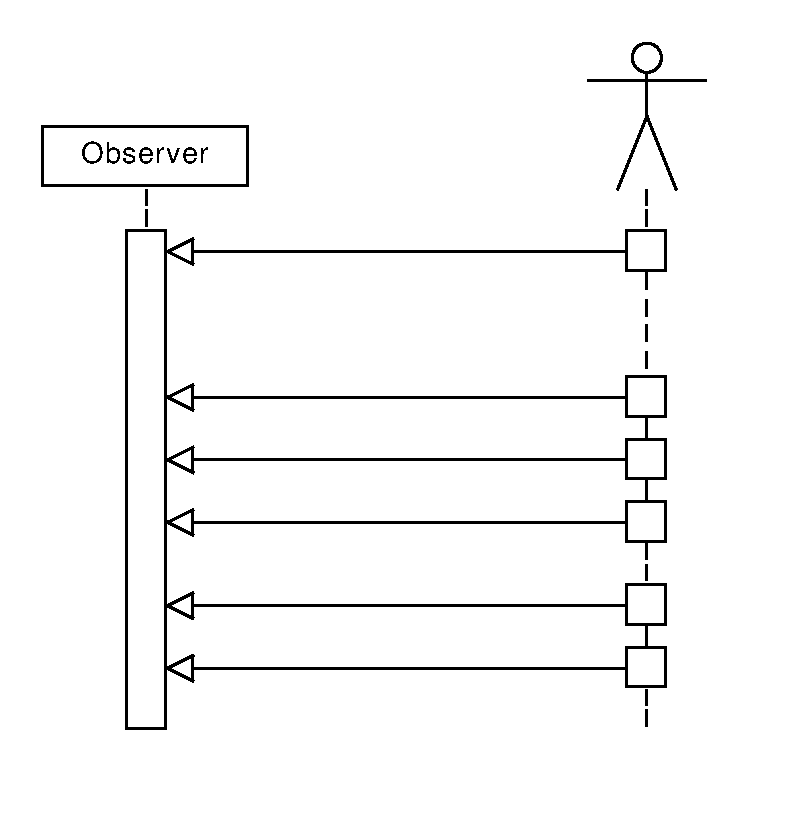
\includegraphics[width=\linewidth]{problem_analysis/opportunistic_sensing}
  \caption{Opportunistic sensing.}
  \label{fig:opportunistic_sensing}
\end{subfigure}
~
\begin{subfigure}[!t]{.45\textwidth}
  \centering
  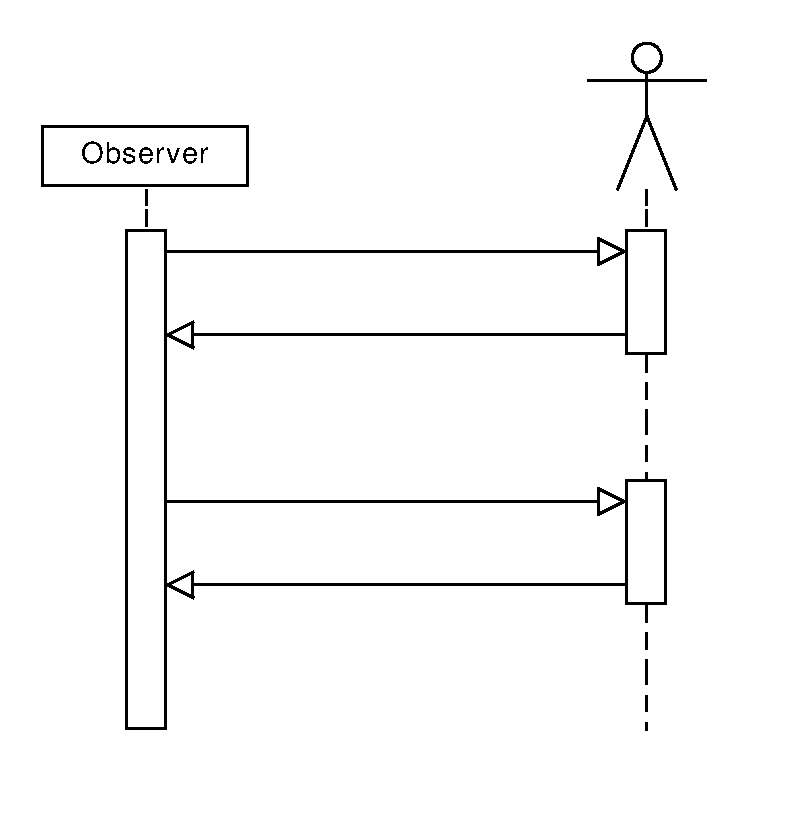
\includegraphics[width=\linewidth]{problem_analysis/participatory_sensing}
  \caption{Participatory sensing.}
  \label{fig:participatory_sensing}
\end{subfigure}
\caption{Two ways of sensing the human activity.}
\label{fig:sensing_types}
\end{figure}
\FloatBarrier

A platform that gathers data for reality mining would have to actively monitor or somehow be aware of when participants are physically located near an area of interest. A configuration of a campaign (it is analogue with the term application query of \parencite{opp_or_par}) could for instance require that data should be gathered when the participant is drinking coffee i.e. they are near a coffee shop. This constant monitoring of the participants context, in order to enable triggers, might though present its own privacy intrusion problems. This monitoring could however be performed strictly locally on the mobile device of the participants and wearables and the participants privacy could thus be somewhat preserved.
\\\\
The two approaches can be combined where opportunistic sensing could then provide context, at opportune times, in the shape of features read from sensors. These features can then be used to learn classes provided from participatory sensing where participants are included to provide the target classes, i.e. labels, in a training data set. Opportunistic sensing could then provide triggers for when participants should be involved in the process. This would allow customers to configure a campaign and specify to which degree they want participant involvement, i.e. participatory sensing, and when and how they want it, i.e. opportunistic sensing.
\\\\
The amount of different classes or labels one could infer directly from the sensor data is somewhat limited and would not allow many possible classes which captures human behavior or state. One could attempt to setup artificial rules and determine the labels in the data based on these rules, these rules would however likely be based on assumptions about the data, unless some other ground truth is known, and it would be difficult to infer many possibly interesting human behavior or state classes for a desired artificial intelligence (AI) model such as for instance stress levels or happiness. One might however with a given algorithm or another machine intelligence model be able to recognize patterns in the data to infer classes, this could for instance be if the person is dancing or not, e.g. by detecting rhythmic movement.    
\\\\
One way to involve participants could be questionnaires with one or more questions. The answers could then determine the labels of the data, or it could be seen as features. The validity of this participant generated data would depend on the truthfulness and perception of the participants which could be a source of error. The validity of the data could however be evaluated and filtered by customers outside the data collection system. Data from external sensors or other certain combinations of values from the collected set of features for each sample, i.e. the participants context, might be helpful in determining the truthfulness of answers provided by participants.
\\\\
We will need to support some kind of participant involvement in order to be able to gather labels for the participants context. The success of the system thus partially depends on how willing participants are to participate, first by actually installing the data gathering application and secondly how actively participants are willing to participate and provide labels for the gathered contexts with respect to the campaigns specified by customers. It is thus up to the customers to design campaigns the participants are willing to participate in. The success of the system thus depends on the ability of the customers, given that the system works as intended.
